\documentclass[dvipsnames, hidelinks]{beamer}

% Enables the use of colour.
\usepackage{xcolor}
% Syntax high-lighting for code. Requires Python's pygments.
\usepackage{minted}
% Enables the use of umlauts and other accents.
\usepackage[utf8]{inputenc}
% Diagrams.
\usepackage{tikz}
% Settings for captions, such as sideways captions.
\usepackage{caption}
% Symbols for units, like degrees and ohms.
\usepackage{gensymb}
% Latin modern fonts - better looking than the defaults.
\usepackage{lmodern}
% Allows for columns spanning multiple rows in tables.
\usepackage{multirow}
% Better looking tables, including nicer borders.
\usepackage{booktabs}
% More math symbols.
\usepackage{amssymb}
% More math layouts, equation arrays, etc.
\usepackage{amsmath}
% More math fonts, like mathbb.
\usepackage{amsfonts}
% More theorem environments.
\usepackage{amsthm}
% More column formats for tables.
\usepackage{array}
% Adjust the sizes of box environments.
\usepackage{adjustbox}
% Better looking single quotes in verbatim and minted environments.
\usepackage{upquote}
% Better blank space decisions.
\usepackage{xspace}
% Better looking tikz trees.
\usepackage{forest}
% URLs.
\usepackage{hyperref}
% For plotting.
\usepackage{pgfplots}

% Various tikz libraries.
% For drawing mind maps.
\usetikzlibrary{mindmap}
% For adding shadows.
\usetikzlibrary{shadows}
% Extra arrows tips.
\usetikzlibrary{arrows.meta}
% Old arrows.
\usetikzlibrary{arrows}
% Automata.
\usetikzlibrary{automata}
% For more positioning options.
\usetikzlibrary{positioning}
% Creating chains of nodes on a line.
\usetikzlibrary{chains}
% Fitting node to contain set of coordinates.
\usetikzlibrary{fit}
% Extra shapes for drawing.
\usetikzlibrary{shapes}
% For markings on paths.
\usetikzlibrary{decorations.markings}
% For advanced calculations.
\usetikzlibrary{calc}

% GMIT colours.
\definecolor{gmitblue}{RGB}{20,134,225}
\definecolor{gmitred}{RGB}{220,20,60}
\definecolor{gmitgrey}{RGB}{67,67,67}

% Change some style options.
\usetheme{metropolis}
\usemintedstyle{manni}
\setbeamercolor{structure}{fg=gmitblue}
\setbeamercolor{frametitle}{fg=white, bg=gmitred}
\setbeamercolor{alerted text}{fg=gmitblue}
\usefonttheme[onlymath]{serif}

% \citeurl can be used to a clickable short url to a slide as a reference.
\renewcommand\footnoterule{}
\newcommand{\citeurl}[1]{\let\thefootnote\relax\footnotetext{\tiny \textcolor{gmitgrey}{\href{http://#1}{#1}}}}

% A basic horizontal rule.
\newcommand{\hr}{\rule{\textwidth}{0.5pt}}

% Prevent minted from showing errors.
\makeatletter
\expandafter\def\csname PYGdefault@tok@err\endcsname{\def\PYGdefault@bc##1{{\strut ##1}}}
\makeatother

\begin{document}
  \title{Turing machines}
  \subtitle{}
  \author{ian.mcloughlin@gmit.ie}
  \date{}

  \begin{frame}
    \titlepage
  \end{frame}

% 1. State tables
% 2. Acceptors
% 3. Tape outputs versus acceptors

\begin{frame}{Visualisation}
  \begin{adjustbox}{max width={0.9\textwidth},center} 
  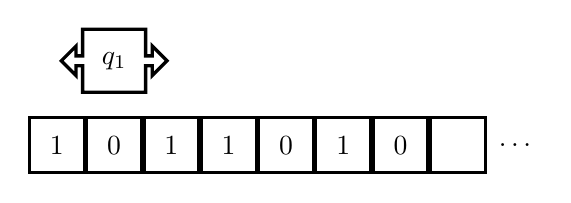
\begin{tikzpicture}
  \tikzstyle{every path}=[very thick]
  
  \edef\sizetape{0.7cm}
  \tikzstyle{tmtape}=[draw,minimum size=\sizetape]
  \tikzstyle{tmhead}=[arrow box,draw,minimum size=.8cm,arrow box arrows={east:.25cm, west:0.25cm}]
  
  \begin{scope}[start chain=1 going right,node distance=-0.15mm]
  \node [on chain=1,tmtape] {1};
  \node [on chain=1,tmtape] (input) {0};
  \node [on chain=1,tmtape] {1};
  \node [on chain=1,tmtape] {1};
  \node [on chain=1,tmtape] {0};
  \node [on chain=1,tmtape] {1};
  \node [on chain=1,tmtape] {0};
  \node [on chain=1,tmtape] {};
  \node [on chain=1,tmtape,draw=none] {$\ldots$};
  \end{scope}

  \node [tmhead,yshift=.7cm] at (input.north) (head) {$q_1$};
  \end{tikzpicture}
  \end{adjustbox}

  \vspace{1.5cm}

  \begin{adjustbox}{max width={0.9\textwidth},center} 
    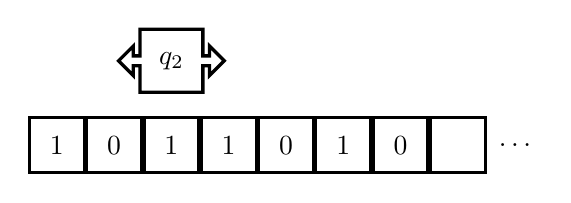
\begin{tikzpicture}
    \tikzstyle{every path}=[very thick]
    
    \edef\sizetape{0.7cm}
    \tikzstyle{tmtape}=[draw,minimum size=\sizetape]
    \tikzstyle{tmhead}=[arrow box,draw,minimum size=.8cm,arrow box arrows={east:.25cm, west:0.25cm}]
    
    \begin{scope}[start chain=1 going right,node distance=-0.15mm]
    \node [on chain=1,tmtape] {1};
    \node [on chain=1,tmtape] {0};
    \node [on chain=1,tmtape] (input) {1};
    \node [on chain=1,tmtape] {1};
    \node [on chain=1,tmtape] {0};
    \node [on chain=1,tmtape] {1};
    \node [on chain=1,tmtape] {0};
    \node [on chain=1,tmtape] {};
    \node [on chain=1,tmtape,draw=none] {$\ldots$};
    \end{scope}
    
    \node [tmhead,yshift=.7cm] at (input.north) (head) {$q_2$};
    \end{tikzpicture}
  \end{adjustbox}
\end{frame}

\begin{frame}{State Table}
  \begin{table}
    \centering
    \begin{tabular}{cc|ccc}
    \toprule
        State & Input & Write & Move & Next \\
    \midrule
        $q_0$ & $\sqcup$ & $\sqcup$ & L & $q_a$ \\
        $q_0$ & 0 & 0 & R & $q_0$ \\
        $q_0$ & 1 & 1 & R & $q_1$ \\
    \midrule
        $q_1$ & $\sqcup$ & $\sqcup$ & L & $q_f$ \\
        $q_1$ & 0 & 0 & R & $q_1$ \\
        $q_1$ & 1 & 1 & R & $q_0$ \\
    \bottomrule
    \end{tabular}
  \end{table}
  

  \[ \delta(q_i, \gamma_n) \rightarrow (q_j, \gamma_m, L/R) \]
\end{frame}



\begin{frame}{Notation}


\begin{description}
  \item[$M$] Turing Machine: $(Q, \Sigma, \Gamma, \delta , q_0, q_a, q_r )$
  \vspace{4mm}
  \item[$Q$] Set of states (finite)
  \item[$\Sigma$] Input alphabet, subset of $\Gamma \setminus \{ \sqcup \} $
  \item[$\Gamma$] Tape alphabet (finite)
  \item[$\sqcup$] Blank symbol, element of $\Gamma$
  \item[$\delta$] Transition function, $\delta: Q \times \Gamma \rightarrow Q \times \Gamma \times \{L,R\}$
  \item[$q_0$] Start state, $\in Q$
  \item[$q_a$] Accept state, $\in Q$
  \item[$q_r$] Reject state, $\in Q$, $\neq q_a$
\end{description}
\end{frame}


\begin{frame}{Blank symbol}

\begin{description}
  \item[Blank] is generally the only difference between the tape alphabet and the input alphabet.
  \item[Definitions] of Turing machines generally don't disallow other symbols in the difference, but there's always at least a blank.
  \item[Empty cells] of the tape in the machine are said to contain the blank symbol.
  \item[Importantly] the blank symbol marks the end of the input on the tape.
  \item[That's why] the input cannot contain the blank symbol.
\end{description}

\end{frame}


\begin{frame}{Sets and alphabets}

\begin{description}
  \item[Recall] sets are just collections of objects called elements.
  \item[Sets] have two important attributes -- an object is either in the set or not, and all elements are distinct.
  \item[Alphabets] in the definition of Turing machines are just sets, and their elements are called symbols.
  \item[Strings] are finite sequences (i.e. ordered lists) of symbols over alphabets.
  \item[$\epsilon$] is the empty string.
  \item[$\mathbb{A}^*$] is the set containing all strings over the alphabet A, including the empty string.
  \item[$|w|$] denotes the length of a string $w$, e.g. if $w = xxyzxy$ then $|w| = 6$.
\end{description}
\end{frame}

\begin{frame}{Alphabets and strings}
\metroset{block=fill}
  \begin{alertblock}{Examples}
    The following are examples of strings over the alphabet $\{0,1\}$:
    \begin{itemize}
      \item 100110
      \item 111
      \item 0
      \item $\epsilon$
    \end{itemize}
  \end{alertblock}
\metroset{block=transparent}
\begin{alertblock}{Single character strings}
Note the distinction between a symbol in an alphabet and the string containing a single string.
They look the same, but one is a symbol and one is a string. 
This is akin to the distinction in C between the character 'a' and the string literal "a".
\end{alertblock}
\end{frame}


\begin{frame}{Languages}

\begin{description}
  \item[Language] is a set of strings.
  \item[Turing machines] accept some strings as inputs.
  \item[Accepted] language of a Turing machine is the set of strings it accepts.
  \item[Halting] -- given a string, a Turing machine will either accept it, reject it, or never stop (fail to halt).
  \item[Decide] -- a Turing machine that halts on all inputs is called a decider for the language it accepts.
  \item[Turing-decidable] -- a language that some Turing machine decides.
\end{description}

\end{frame}



\begin{frame}{Turing's Second Example}
  \begin{quote}
    As a slightly more difficult example we can construct a machine to compute the sequence $001011011101111011111\ldots$.
    The machine is to be capable of five $m$-configurations, viz. $\mathfrak{o}$, $\mathfrak{q}$, $\mathfrak{p}$, $\mathfrak{f}$, $\mathfrak{b}$ and of printing $e$, $x$, $0$, $1$.
    The first three symbols on the tape will be $ee0$; the other figures follow on alternate squares.
    On the intermediate squares we never print anything but $x$.
    These letters serve to keep the place for us and are erased when we have finished with them.
    We also arrange that in the sequence of figures on alternate squares there shall be no blanks.
  \end{quote}
  \citeurl{www.cs.virginia.edu/~robins/Turing\_Paper\_1936.pdf}
\end{frame}



\begin{frame}{Turing's Second Example: Table}
  \begin{table}
  \resizebox{\textwidth}{!}{
    \centering
    \begin{tabular}{cccc}
      \emph{m-config.}  & \emph{symbol}  & \emph{operations} & \emph{final m-config.} \\
      $\mathfrak{b}$ & & $Pe,R,Pe,R,P0,R,R,P0,L,L$  & $\mathfrak{o}$ \\
      & & & \\
      \multirow{2}{*}{$\mathfrak{o}$} & $1$ & $R,Px,L,L,L$ & $\mathfrak{o}$ \\
      & 0 & & $\mathfrak{q}$ \\
      & & & \\
      \multirow{2}{*}{$\mathfrak{q}$} & Any (0 or 1) & $R,R$ & $\mathfrak{q}$ \\
      & None & $P1,L$ & $\mathfrak{p}$ \\
      & & & \\
      \multirow{3}{*}{$\mathfrak{p}$} & x & $E,R$ & $\mathfrak{q}$ \\
      & e & R & $\mathfrak{f}$ \\
      & None & $L,L$ & $\mathfrak{p}$ \\
      & & & \\
      \multirow{2}{*}{$\mathfrak{f}$} & Any & $R,R$ & $\mathfrak{f}$ \\
      & None & $P0,L,L$ & $\mathfrak{o}$ \\
    \end{tabular}}
  \end{table}
\end{frame}


\begin{frame}[fragile]{Turing's Second Example: Initial state and tape}
\begin{minted}{javascript}
// The contents of the tape.
var tape = [];
// The current position of the machine on the tape.
var pos = 0;
// The current state.
var state = b;
\end{minted}
\end{frame}

\begin{frame}[fragile]{Turing's Second Example: Reading and writing}
\begin{minted}{javascript}
// The blank symbol.
var blank = undefined;

// Write symbol sym to the current cell on the tape.
function write(sym) {
	tape[pos] = sym;
}

// Return true iff the symbol in the current cell is sym.
function read(sym) {
	return sym == tape[pos] ? true : false;
}
\end{minted}
\end{frame}

\begin{frame}[fragile]{Turing's Second Example: Moving the machine}
\begin{minted}{javascript}
// Move the machine head right.
function right() {
	pos++;
}

// Move the machine head left.
function left() {
	pos--;
}
\end{minted}
\end{frame}


\begin{frame}[fragile]{Turing's Second Example: State b}
\begin{table}
    \centering
    \begin{tabular}{cccc}
      \emph{m-config.}  & \emph{symbol}  & \emph{operations} & \emph{final m-config.} \\
      $\mathfrak{b}$ & & $Pe,R,Pe,R,P0,R,R,P0,L,L$  & $\mathfrak{o}$
    \end{tabular}
  \end{table}

\begin{minted}{javascript}
function b() {
	write('e'); right();
	write('e'); right();
	write('0'); right(); right();
	write('0'); left(); left();
	state = o;
}
\end{minted}
\end{frame}


\begin{frame}[fragile]{Turing's Second Example: State q}
\begin{table}
    \centering
    \begin{tabular}{cccc}
      \emph{m-config.}  & \emph{symbol}  & \emph{operations} & \emph{final m-config.} \\
      \multirow{2}{*}{$\mathfrak{q}$} & Any (0 or 1) & $R,R$ & $\mathfrak{q}$ \\
      & None & $P1,L$ & $\mathfrak{p}$ \\
    \end{tabular}
  \end{table}

\begin{minted}{javascript}
function q() {
	if (read('0') || read('1')) {
		right(); right(); state = q;
	}
	else if (read(blank)) {
		write('1'); left(); state = p;
	}
}
\end{minted}
\end{frame}


\end{document}
 
